\section{Word embeddings}
\label{sec:word-embeddings}
In this section, we will formulate the problem of creating efficient vectorized representations of text and explain methods for doing so. In particular, we will discuss ways of representing text numerically in \cref{sec:numerical-repr-of-text}, describe how we can create word embeddings and details around the word2vec method in \cref{sec:word2vec}, from architectural choices to presenting word2vec as an artificial neural network. Finally, we will introduce a couple of alternative models for learning word embeddings in \cref{sec:other-models-for-learning-word-embeddings} and explain how to evaluate word embedding models in \cref{sec:eval-word-embedding-models}.

\subsection{Numerical representation of text}
\label{sec:numerical-repr-of-text}
Machine learning methods take in vectors (arrays of numbers) as input. When we want to work with text, we have to come up with some procedure for converting text into a vector, i.e. vectorizing the text. In this subsection, we create unique representations for words in a text, discuss one-hot encoding of words and the motivation behind creating word embeddings.

\subsubsection{Unique representation for each word}
\label{unique-representation-for-each-word}
A first strategy for vectorizing text could be to assign a unique number for each word in the text. We use the same order as the words that appear in the text to assign a unique number. We call the set of unique words that appear in the text the \textit{vocabulary} and denote it as $V$. Furthermore, we define the number of unique words in the text to be the \textit{vocabulary size} and denote it as $|V|$. Finally, we replace each word in the text with its respective number. Let us consider an example of a (lower-cased) sentence, which we define as
\begin{align}
    S = \text{the cat sat on the mat}.
    \label{eqn:num-rep-ex-sent-words}
\end{align}

Following, we convert the words into numbers using the numerical order they appear in the text, e.g. the $\mapsto$ 0, cat $\mapsto$ 1, sat $\mapsto$ 2, etc. We convert the sentence in \cref{eqn:num-rep-ex-sent-words} to numbers as
\begin{align}
    S = \text{0 1 2 3 0 4}
    \label{eqn:num-rep-ex-sent}.
\end{align}
In \cref{eqn:num-rep-ex-sent}, we see a numerical representation of the original sentence in \cref{eqn:num-rep-ex-sent-words} and may use it for machine learning modeling. However, there are some problems with this method:
\begin{itemize}
    \item The encoding of words into number is arbitrary (does not capture any relationship between words)
    \item Machine learning models might learn some natural ordering of the encodings, which can lead to bad results during inference. This is because the encoding of the words does not capture the relationship between the words.
\end{itemize}

In the next sub-subsection, we look at another method for encoding words, using one-hot encodings. Furthermore, we apply it to the example sentence in \cref{eqn:num-rep-ex-sent-words}.

\subsubsection{One-hot encoded words}
\textit{One-hot encoding} is a method for converting categorical data into numeric data. Essentially, we create a unique, sparse vector consisting of all zeros, except for the value at the index of the element of interest, which we set to one. For instance, if we have the words "north", "east", "south", "west", then their one-hot encodings could be
\begin{align}
    \text{north} \mapsto \begin{pmatrix}
    1\\
    0\\
    0\\
    0
    \end{pmatrix},
    \text{east} \mapsto \begin{pmatrix}
    0\\
    1\\
    0\\
    0
    \end{pmatrix},
    \text{south} \mapsto \begin{pmatrix}
    0\\
    0\\
    1\\
    0
    \end{pmatrix},
    \text{west} \mapsto \begin{pmatrix}
    0\\
    0\\
    0\\
    1
    \end{pmatrix}.
\end{align}

Let the vocabulary $V = \left \{ w_1, w_2, ..., w_{|V|} \right \}$ to be the set of unique words in a text. Then, we define the one-hot encoding of a word, $e_{w_i}$, to be the $|V|$-dimensional vector of all zeros, except for the value at index $i$ which is one. Using the definition of one-hot encoding, we convert the words from the sentence in \cref{eqn:num-rep-ex-sent-words}. Precisely, we convert the sentence as
\begin{align}
    S = \begin{pmatrix}
    1\\
    0\\
    0\\
    0\\
    0
    \end{pmatrix}
    \begin{pmatrix}
    0\\
    1\\
    0\\
    0\\
    0
    \end{pmatrix}
    \begin{pmatrix}
    0\\
    0\\
    1\\
    0\\
    0
    \end{pmatrix}
    \begin{pmatrix}
    0\\
    0\\
    0\\
    1\\
    0
    \end{pmatrix}
    \begin{pmatrix}
    1\\
    0\\
    0\\
    0\\
    0
    \end{pmatrix}
    \begin{pmatrix}
    0\\
    0\\
    0\\
    0\\
    1
    \end{pmatrix},
    \label{eqn:one-hot-rep-ex-sent-words}
\end{align}
where we see that we discard the the ordinal relationship of the numerical representation in \cref{eqn:num-rep-ex-sent}. However, there are some downsides with this approach, as well:
\begin{itemize}
    \item As with the numerical representation in \cref{unique-representation-for-each-word}, one-hot encoded vectors does not capture the relationship between words.
    \item One-hot encoded vectors are sparse (meaning, most values are zero). Imagine if we had 1000 words in the vocabulary, then one would create a vector consisting of 99.9\% zeros. In practice, the vocabulary size is in the terms of $10^5$ to $10^7$ \cite{mikolov2013b}, i.e. by using one-hot encoded vector representations we are extremely inefficient in terms of space. We note, however, that there exist efficient methods for dealing with sparse vectors.
    \item One-hot encoded vectors are very high-dimensional (same as the number of words in the vocabulary, $|V|$).
\end{itemize}
In the next sub-subsection, we look at word embeddings, which solves many of the problems of the numerical representations presented so far.

\subsubsection{Word embeddings}
In comparison to the high-dimensional one-hot encoded vectors of words, \textit{word embeddings} are low-dimensional dense vector representations. Word embedding models learn their word embeddings from the data (e.g. texts) directly, whereas, for one-hot encoded vectors, we can arbitrarily define them (e.g. its ordering may change). Also, due to the lower dimensionality of word embeddings, it has to pack more information about words into less space. Moreover, word embeddings use all their dimensions to learn hidden relations and concepts of words, in contrast to one-hot encodings, which effectively only uses a single dimension (e.g. the position of the word in the vocabulary). Common choices for the dimensionality of word embeddings range from 50 to 600 \cite{mikolov2013a}, depending on the amount of training data. In the next subsection, we look at a classic family of methods for creating such word embeddings, namely word2vec.

\subsection{Learning word embeddings}
\label{sec:word2vec}
\textit{Word2vec} was first introduced by Mikolov et al. in 2013 \cite{mikolov2013a}. It is a family of methods for learning dense and efficient vector representations of words. In the same year, Mikolov et al. published a follow-up paper, \cite{mikolov2013b}, which includes several extensions that improve both the quality of the word embeddings and the training speed. In this subsection, we explain the details of the original word2vec paper, \cite{mikolov2013a}, and the introduced extensions in the follow-up paper, \cite{mikolov2013b}. We base this subsection on \cites{mikolov2013a}{mikolov2013b}. Furthermore, we will use the word2vec method to create word embeddings for the analysis in \cref{sec:training-and-eval-our-word2vec-impl}.

\subsubsection{Architectures}
The authors of the word2vec paper introduced two new log-linear models for learning distributed representations of words that try to minimize computational complexity, namely the \textit{continuous bag-of-words model} (CBOW) and the \textit{continuous Skip-gram model}. Both models achieve high quality (see \cref{sec:eval-word-embedding-models} for evaluation of word2vec models) word embeddings and share some core idea as to how we can create good vector representations of words. In this sub-subsection, we go through both models and explain the similarities and differences.

\paragraph*{Continuous bag-of-words model}\mbox{} \\
The continuous bag-of-words model (CBOW) tries to predict a target word given some context words around it. Essentially, we select a target word $w_t$, where $t$ is the index of the current target word in our training data, and a number $C$ denoting the number of words to the left and the right of $w_t$. We also refer to $C$ as the \textit{window size}. Let $S=2C$ denote the total number of words to the left and right. By combining the context word embeddings, we predict the target word $w_t$. We illustrate the CBOW model in \cref{fig:cbow-model}.
\begin{figure}[H]
    \centering
    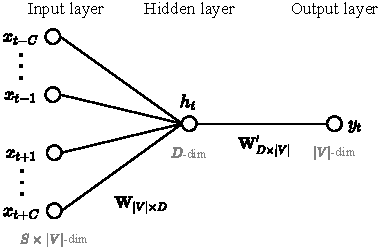
\includegraphics[width=11cm]{thesis/figures/cbow_cropped.pdf}
    \caption{An illustration of the CBOW architecture. The input value $x_{t+k}$ is the one-hot encoded vector of word $w_{t+k}$, where $k \in \enclc{-C, \ldots, -1, 1, \ldots, C}$, $t \in \enclc{1, \ldots, T}$ is training word position and $C$ is the window size. The output of CBOW is a $|V|$-dimensional vector $y_t$ of probabilities for sampling the target word $w_t$.}
    \label{fig:cbow-model}
\end{figure}

More formally, we are considering a sequence of $T$ training words $w_1, w_2, \ldots, w_T$. The words $w_t$ belong to some vocabulary $V$ consisting of $|V|$ unique words, $1 \leq t \leq T$. The models task is to maximize the average log probability of sampling the word $w_t$, given the context words $w_{t-C}, \ldots, w_{t-1}, w_{t+1}, \ldots, w_{t+C}$. The objective of the CBOW model then becomes
\begin{align}
    \frac{1}{T} \sumlim{t=1}{T} \log p(w_t | w_{t-C}, \ldots, w_{t-1}, w_{t+1}, \ldots, w_{t+C}).
    \label{eqn:cbow-objective-function}
\end{align}

Through it is not clear from the original authors of word2vec \cite{mikolov2013a, mikolov2013b}, we typically use two weight matrices, $W$ and $W'$, when setting up the word2vec model \cite{rong2016word2vec}. The first weight matrix, $W$, is a $|V| \times D$ matrix, mapping the input words (we typically represent them using one-hot encodings) to their internal word embeddings, where $|V|$ is the vocabulary size, and $D$ is the number of dimensions in the embedding layer. The second weight matrix, $W'$, is a $D \times |V|$ matrix mapping from the embedding layer to the output prediction. In practice, we use the first weight matrix $W$ as word embeddings, but we note that some models utilize both weight matrices (e.g. GloVe in \cref{sec:glove}).

\paragraph*{Continuous Skip-gram model}\mbox{} \\
The continuous Skip-gram model is very similar to CBOW, and in fact, the Skip-gram model tries to do the opposite; instead of predicting a target word given some context words, it tries to predict context words given some target word. We note that the ordering of the predicted context words does not matter. We illustrate the Skip-gram model in \cref{fig:skip-gram-model}.
\begin{figure}[H]
    \centering
    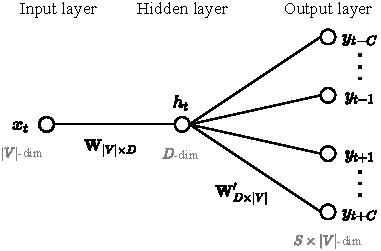
\includegraphics[width=11cm]{thesis/figures/skim-gram_cropped.pdf}
    \caption{An illustration of the Skip-gram architecture. The input value $x_t$ is the one-hot encoded vector of word $w_t$, where $t \in \enclc{1, \ldots, T}$ is training word position and $C$ is the window size. The output values are $|V|$-dimensional vectors $y_{t+k}$ of probabilities for sampling the word $w_{t+k}$, where $k \in \enclc{-C, \ldots, -2, -1, 1, 2, \ldots, C}$. We note that the ordering of the vectors from the output layers does not matter, as we only want to predict that a particular word belongs to its contextual words.}
    \label{fig:skip-gram-model}
\end{figure}

With the Skip-gram model, we also have some target word $w_t$ and context words around it. Let $C$ be the maximal distance from a target word to its contextual words. For each input to the model, we randomly sample a number $R$ in the range $[1, C]$ and denote this as the \textit{context size}. In other words, for each target word $w_t$ we have $R$ context words around it, $w_{t-R}, \ldots, w_{t-1}, w_{t+1}, \ldots, w_{t+R}$. The objective of the Skip-gram model then becomes
\begin{align}
    \frac{1}{T} \sumlim{t=1}{T} \sumlim{-R \leq j \leq R, j \neq 0}{} \log p(w_{t+j} | w_t).
    \label{eqn:skip-gram-objective-function}
\end{align}
More generally, we define the objective of the Skip-gram model as such
\begin{align}
    \frac{1}{T} \sumlim{t=1}{T} \sumlim{w_O \in cw(w_I)}{} \log p(w_O | w_I),
    \label{eqn:skip-gram-objective-function-general}
\end{align}
where $w_I$ is the input word (e.g. target word), $w_O$ is the output word (e.g. context word) and $cw(w_I)$ is a function which returns the context words around input word $w_I$.

Similar to CBOW, the Skip-gram model uses the two matrices $W$ and $W'$ for mapping from input to embedding layer and embedding layer to output respectively. Mikolov et al. report that the Skip-gram model performs better than the CBOW model overall, shown by their experiments in \cites{mikolov2013a}. For this reason, and due to the scope of the thesis, we will focus on the Skip-gram model. For the rest of the thesis, we refer to the weight matrix $W$ when talking about word embeddings of a word2vec model.

\subsubsection{Negative Sampling}
In the Skip-gram model, we typically compute $p(w_O | w_I)$ using the softmax function (see \cref{eqn:softmax-function}). More formally, we define it as
\begin{align}
    p(w_O | w_I)
    &= \frac{\exp{ \left( \trans{v'_{w_O}} v_{w_I} \right) }} {\exp{ \sumlim{k=1}{|V|} \left( \trans{v'_{w_k}} v_{w_I} \right) }},
    \label{eqn:skip-gram-p-function}
\end{align}
where $v_w$ and $v'_w$ are the "input" and "output" vector representations of the word $w$, and $|V|$ is the number of words in the vocabulary. There are some downsides with this formulation, however. In practice, it becomes hard to compute since the summation in the denominator of \cref{eqn:skip-gram-p-function} depends on the number of words in the vocabulary, which is often large ($10^5 - 10^7$ terms).

To deal with the computational requirements of the original Skip-gram model, \cite{mikolov2013b} first show that using \textit{hierarchical softmax}, we end up with a viable strategy. Hierarchical softmax is an efficient way of computing the softmax function; instead of evaluating $|V|$ words to compute the probability in \cref{eqn:skip-gram-p-function}, we only have to evaluate $\log \left( |V| \right)$ words.

As an alternative to hierarchical softmax, Mikolov et al. introduced \textit{negative sampling} in \cite{mikolov2013b}. Negative sampling builds on the concept of distinguishing target words $w_t$ from words randomly sampled from the vocabulary. In particular, we randomly sample words from the vocabulary using the \textit{unigram distribution} raised to the power of $\alpha$. The unigram distribution is a distribution used to sample random words from the vocabulary using the word occurrence counts. \cite{mikolov2013b} claim that by raising the unigram distribution to the power of $\alpha = 3/4$, we get the best result. Furthermore, we refer to this unigram distribution as the noise distribution $P_n(w)$. Note that we can also apply the negative sampling method to CBOW, but we leave these details out.

Before we can explain negative sampling, we define the positive and negative target-context pairs. Given a vocabulary $V$, a target word $w_t$ and the target words contextual words $w_{t-R}, \ldots, w_{t-1}, w_{t+1}, \ldots, w_{t+R}$ for some window size $R$, we define a \textit{positive target-context pair} to be the pair of the target word $w_t$ and a contextual word $w_{t+j}$, $-R \leq j \leq R, j \neq 0$, i.e. the pair $\left( w_t, w_{t+j} \right)$. Furthermore, we define a \textit{negative target-context pair} as the pair of the target word $w_t$ and a word $w_r$, i.e. the pair $\left( w_t, w_r \right)$. We randomly sample the word $w_r$ from the noise distribution $P_n(w)$.

To explain the idea of negative sampling, we look at how we compute the softmax loss, and in particular, how we only use a subset of all the words in the vocabulary. In particular, for each word in the text we are training on, we create a positive target-context pair $\left( w_t, w_{t+j} \right)$, $-R \leq j \leq R, j \neq 0$. Furthermore, we generate $k$ negative target-context pairs for each word, where $k$ is in the range of $5-20$ for small training sets and $2-5$ for big training sets. We let $W_{np} = \left \{ w_i | i \in 1, \ldots, k \right \}$ be the set of $k$ negatively sampled words from the noise distribution $P_n(w)$. With these details in mind, the objective of negative sampling becomes \cite{mikolov2013b, rong2016word2vec}
\begin{align}
    \log \sigma \left( \trans{v'_{w_O}} v_{w_I} \right) + \sumlim{w_i \in W_{np}}{} \log \sigma \left( -\trans{v'_{w_i}} v_{w_I} \right),
    \label{eqn:negative-sampling-obj-func}
\end{align}
where $\sigma$ is the sigmoid function (see \cref{eqn:sigmoid-function}), and $v_t$ and $v'_t$ are the "input" and "output" vector representations of the word $w$. Note that the objective in \cref{eqn:negative-sampling-obj-func} can be seen as a special case of the negative cross-entropy loss function. Furthermore, we replace every $\log p(w_O | w_I)$ in the original Skip-gram objective function of \cref{eqn:skip-gram-objective-function-general} by the objective in \cref{eqn:negative-sampling-obj-func}. As such, we define the objective of the Skip-gram model with negative sampling as
\begin{align}
    \frac{1}{T} \sumlim{t=1}{T} \sumlim{w_O \in cw(w_I)}{} \log \sigma \left( \trans{v'_{w_O}} v_{w_I} \right) + \sumlim{w_i \in W_{np}}{} \log \sigma \left( -\trans{v'_{w_i}} v_{w_I} \right).
    \label{eqn:skip-gram-negative-sampling-objective}
\end{align}
In \cref{eqn:negative-sampling-obj-func}, we see that we only have to compute for $(1 + k)$ words, which is a big improvement over computing for $|V|$ words (assuming that $|V|$ is much larger than $k$). \cites{mikolov2013b} also report that by using negative sampling, we increase the quality of the word embeddings.

\subsubsection{Subsampling of words}
When training a word2vec model, we typically have to train on big text corpora to achieve high-quality word embeddings. However, as the number of training words increases, the discrepancy between rare and frequent words increase as well. When using negative sampling, we are sampling negative target-context pairs from the vocabulary, which depends on the unigram distribution. In English text corpora, words such as "the", "of", "is" can easily occur hundreds of millions of times and usually provide less information than more rare words. For this reason, we apply a simple, yet efficient subsampling scheme to counter the imbalance between rare and frequent words; before we process the text corpora into target-context pairs, we discard each word $w_t$ with a \textit{discard probability} \cite{mikolov2013b, levy-etal-2015-improving}. We define the discard probability as
\begin{equation}
    P_d(w_t) = 1 - \sqrt{\frac{t}{f(w_t)}},
\end{equation}
where $f(w_t)$ is the (relative) frequency of word $w_t$ and $t$ is a chosen threshold, usually around $10^{-5}$.

We note, however, that in the original source code of word2vec \cite[line 407]{Word2vecCCode}, they use a slightly modified formula. We define the modified formula as 
\begin{align}
    P_d(w_t) = \frac{f(w_t) - t}{f(w_t)} - \sqrt{\frac{t}{f(w_t)}}.
    \label{eqn:discard-probability-impl}
\end{align}
Furthermore, we will use subsampling of words when implementing word2vec in \cref{sec:training-and-eval-our-word2vec-impl}, and in particular, we will use \cref{eqn:discard-probability-impl} for computing the discard probability.

\subsubsection{Learning word embeddings for phrases}
\label{sec:learning-word-embeddings-for-phrases}
Phrases are groups of words that occur frequently together, such as "New York" or "programming languages". Naturally, we would like to combine such words into a single token, such that word embedding models can learn them. To learn word embeddings for phrases, \cite[4 Learning Phrases]{mikolov2013b} propose a simple, yet efficient data-driven approach, where they combine phrases using their word counts. In particular, we define the phrase score for two words $w_i$ and $w_j$ as
\begin{align}
    \text{score}(w_i, w_j) = \frac{\text{freq}(w_i, w_j) - \delta}{\text{freq}(w_i) \cdot \text{freq}(w_j)},
    \label{eqn:word2phrase-score}
\end{align}
where $w_i$ and $w_j$ are bigrams, or two neighbouring words, from the vocabulary, $freq()$ returns the how many times the word (or bigram) occurs in the vocabulary and $\delta$ is a hyperparameter for preventing long phrases consisting of infrequent words from appearing. We refer to this phrase-learning procedure as \textit{word2phrase}, as specified by the original source code \cites{Word2phraseCCode}. If the score in \cref{eqn:word2phrase-score} is above the $\delta$ threshold hyperparameter, we accept the bigram into the vocabulary and we replace all occurrences of the two words $w_i$ and $w_j$ where they are next to each other. We use word2phrase to convert phrases into single words when preprocessing data for training our word2vec model in \cref{sec:word2vec-data-preprocessing}.

\subsubsection{Word2vec as an artificial neural network}
\label{sec:word2vec-as-an-ann}
Typically in the literature, word2vec is presented using the \cref{eqn:cbow-objective-function,eqn:skip-gram-p-function,eqn:negative-sampling-obj-func}. However, we explain how to set word2vec up as an artificial neural network (ANN, \cref{sec:artificial-neural-networks}), in the sense that we implement it later in the thesis (see \cref{sec:training-and-eval-our-word2vec-impl}). In particular, we explain how to set up the Skip-gram model with negative sampling as an ANN. This ANN consists of three fully-connected layers of artificial neurons \cite{rong2016word2vec}, and we illustrate it in \cref{fig:word2vec-skip-gram-negative-sampling}. The ANN we explain below acts as a baseline when implementing word2vec in \cref{sec:word2vec-impl-specifics}.

\begin{figure}[ht]
    \centering
    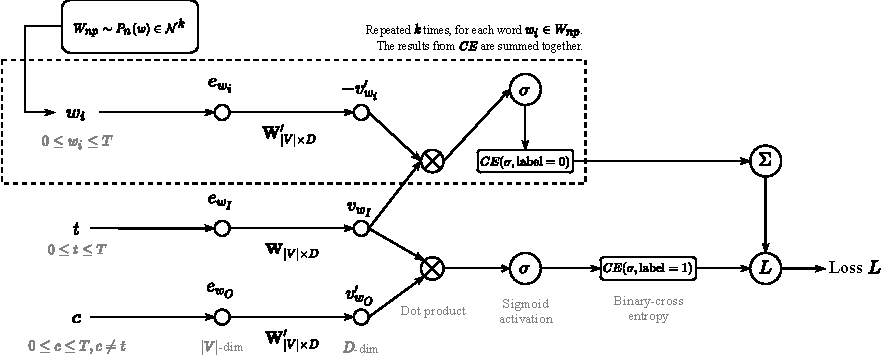
\includegraphics[width=16cm]{thesis/figures/word2vec-sgns_cropped.pdf}
    \caption{The artificial neural network architecture of word2vec Skip-gram model with negative sampling. The inputs to the network are $t$ and $c$, i.e, index of target word $w_t$ and context word $w_c$ in the vocabulary. For each forward pass in the network we sample $k$ word indices from $P_n(w)$. Furthermore, we use the $k$ sampled word indices to compute the negative sampling loss $L$.}
    \label{fig:word2vec-skip-gram-negative-sampling}
\end{figure}

\paragraph*{Input layers}\mbox{} \\
We have two input layers in our ANN; one for the target word $w_t$ and one for the context word $w_{t+j}$, $-R \leq j \leq R, j \neq 0$. The values to the input layers are typically one-hot encoded or represented using an integer corresponding to the index of the word in the vocabulary. For explanation purposes, we use the one-hot encoded representation here, but in our code implementation, we will use the latter one. We denote the input layers to be $\enclc{e_{w_t}}$ for the target word $w_t$ and $\enclc{e_{w_{t+j}}}$ for the context word $w_{t+j}$. Each of the input layers has $|V|$ values, where $|V|$ is the size of the word vocabulary.

\paragraph*{Hidden layer}\mbox{} \\
We have one hidden layer for each input layer in our ANN. To calculate the result from the input layers to its hidden layer, we introduce two $D \times |V|$ weight matrices $W$ and $W'$, where $D$ is the hidden embedding dimension and $|V|$ is the vocabulary size. The $W$ matrix consists of weights related to the target word $w_t$ and can be thought of as the "input to hidden" matrix. The $W'$ matrix consists of weights related to the context word, and unlike the $W$ matrix, it can be thought of as the "hidden to output" matrix from the original introduction to negative sampling. Note that we initialize both $W$ and $W'$ at random. Furthermore, we refer to $W$ and $W'$ as the target and context embedding matrix, respectively.

To map from the input to the hidden layer, we use a linear activation function (i.e. $id(x) = x$) with no bias, leading to more efficient training of bigger datasets. In other words, we simply multiply the embedding matrix (either $W$ or $W'$) with its respective one-hot encoded input vector, resulting in a "look-up" of the embedding vector. To illustrate with an example, imagine if we had the one-hot encoded vector $e_{w_t} = \left( \begin{smallmatrix}
    1\\
    0\\
\end{smallmatrix} \right)$ and the embedding matrix $W = \trans{\left( \begin{smallmatrix}
    1 & 2 & 3\\
    4 & 5 & 6\\
\end{smallmatrix} \right)}$. If the multiply the embedding matrix with the one-hot encoded vector, i.e. $W \cdot e_{w_t}$, we would get $\trans{\left( \begin{smallmatrix}
    1 & 2 & 3\\
\end{smallmatrix} \right)}$, essentially performing a "copy" operation. We let $\enclc{v_{w_t}} = W \cdot \enclc{e_{w_t}}$ be the hidden layer for word $w_t$ and $\enclc{v'_{w_{t+j}}} = W' \cdot \enclc{e_{w_{t+j}}}$ be the hidden layer for word $w_{t+j}$. 

\paragraph*{Output layer}\mbox{} \\
Recall that when we are using negative sampling, we would like to ensure that words in the same context yield similar word embeddings, and that words that are not in the same context (i.e. a target word versus a word sampled from the noise distribution $P_n(w)$) to be dissimilar. From the objective of negative sampling in \cref{eqn:negative-sampling-obj-func}, we see that we use the sigmoid function on the dot product between the "input" and the "output" vectors $v$ and $v'$ (in our setting: $\enclc{v_{w_t}}$ and $\enclc{v'_{w_{t+j}}}$). When we take the dot product, we are essentially computing an unnormalized cosine similarity measure between the vectors (we come back to the use of cosine similarity in \cref{sec:eval-word-embedding-models}). The core idea is to use this dot product similarity measure and convert it into the range of $[0, 1]$ by using the sigmoid function. Particularly, we want similar vectors to have 1 as output from the sigmoid function and dissimilar vectors to have 0 as the output from the sigmoid function. When we compute the loss of the ANN, we generate $k$ samples from the noise distribution $P_n(w)$ such that we can use them for computing the loss of the network.

For each positive target-context pair we have in our data, we create a single sigmoid output plus $k$ sigmoid outputs for each negative word we sample from the noise distribution $P_n(w)$. Thus, we could argue that we have $(k + 1)$ outputs in our network.  We note that, however, our main interest is to learn the internal embedding matrix $W$; we do not use the ANN for predicting whether a certain word is more or less likely to be within its contextual neighbourhood, thus, discarding the output of the network.

Similar to \cite{mikolov2013a}, we update the embedding weights $W$ and $W'$ using the stochastic gradient descent optimizer (see \cref{sec:ann-optimizers}), adjusting all the weights of the embedding matrices during the training of the ANN to minimize the loss in \cref{eqn:skip-gram-negative-sampling-objective}. Furthermore, we use a linearly decreasing learning rate, meaning that we start with some initial learning rate $lr$ and decrease linearly to $lr_{min}$ until we reach the end of training. The linearly decreasing learning rate is also used by \cite{mikolov2013a}.

\subsubsection{Hyperparameters in word2vec}
When training a word2vec model, we have to choose several hyperparameters. In this sub-subsection, we go over all choices of hyperparameters and explain them. We will explain the specific choices of hyperparameters that we use to train a word2vec model in \cref{sec:word2vec-hyperparameter-choices}.

\begin{itemize}
    \item \textbf{min-word-count} \\
        The minimum word count denotes a threshold of how many times a word at least has to occur in a text for it to be in the vocabulary. In the empirical experiments of Mikolov et al, they used 5 as the threshold.
    \item \textbf{max-vocab-size} \\
        The maximum vocabulary size denotes the maximal number of words to have in our vocabulary; we use the top \textbf{max-vocab-size} most common (i.e frequent) words. We may set the maximum vocabulary size to reduce the computational complexity and to remove some less occurring words.
    \item \textbf{batch-size} \\
        Batch size is the number of positive target-context pairs $(w_t, w_{t+j})$ we train on in each training step, i.e. the number of forward passes we perform in our ANN before we do a backwards pass.
    \item \textbf{num-epochs} \\
        The number of epochs denotes the number of times we train on the training data. With word2vec, we typically set this number rather low (e.g. $1-5$), as \cites{mikolov2013a} reports that by training on more data, we require fewer epochs to get comparable or better quality word embeddings.
    \item \textbf{learning-rate} \\
        The learning rate denotes how fast we want our weights to change in our ANN. The original authors of word2vec used 0.025 (i.e. $2.5\%$) as the initial learning rate for their experiments.
    \item \textbf{min-learning-rate} \\
        The minimal learning rate denotes how small the learning rate should be when approaching the end of the training. Mikolov et al. stated that they decreased it linearly, such that it approaches zero at the end of the last training epoch. We note, however, that in the original code of word2vec, they linearly decrease the learning rate to the initial learning rate $lr$ times $0.0001$ (i.e. $0.025 \times 0.0001 = 0.0000025$) \cite[line 398]{Word2vecCCode}.
    \item \textbf{embedding-dim} \\
        The embedding dimension denotes the dimension we want to use for the internal matrices $W$ and $W'$ in our ANN, i.e. the dimensionality of the word embeddings.
    \item \textbf{max-window-size} \\
        Maximum window size denotes the maximal number of words to look for to the left and the right of a target word $w_t$. Mikolov et al. reported that they used $5$ as the window size.
    \item \textbf{num-negative-samples} \\
        The number of negative samples denotes how many negative samples we generate for each positive target-context pair we train on.
    \item \textbf{sampling-factor} \\
        We use the sampling factor as a threshold to randomly discard frequently occurring words in the text corpora. A common value for this is $10^{-5}$.
    \item \textbf{unigram-exponent} \\
        The unigram exponent is which power we raise the noise distribution $P_n(w)$ to (where the noise distribution equals the unigram distribution, in our case). Although there was no theoretical justification for this, Mikolov et al. reported that the value $3/4$ worked the best.
\end{itemize}

\subsection{Other models for learning word embeddings}
\label{sec:other-models-for-learning-word-embeddings}
Creating word embeddings is a task that can be achieved in various ways. In this subsection, we briefly introduce two different models for computing word embeddings. The first model is the Global Vectors (GloVe) \cite{pennington2014glove} model. GloVe learns vector representations for words in a more "explicit" fashion than word2vec for example; we come back to this in \cref{sec:glove}. The second model is the fastText \cite{bojanowski2017enriching} model, which is an extension of the original word2vec Skip-gram model to include sub-word information. Note that we primarily focus on word2vec using Skip-gram with negative sampling in this thesis, and for this reason, we not go into depth when explaining GloVe and fastText. We will use pre-trained GloVe and fastText models when comparing evaluation results of word embedding models in \cref{sec:word2vec-model-evaluation} and when we analyze word embeddings in \cref{sec:analysis-of-embeddings-topological-polysemy}.

\subsubsection{GloVe}
\label{sec:glove}
\textit{Global Vectors} (GloVe) \cite{pennington2014glove} is a model for learning vector representations for words. In contrast to word2vec, GloVe trains on the word to word co-occurrence counts, and thus, makes efficient use of statistics. In addition to this, the objective of GloVe is more explicit, as opposed to the vector representations word2vec learns, which are merely a by-product of the training. We base this sub-subsection on \cite{pennington2014glove}.

To understand how GloVe works, we first introduce the notion of the \textit{word to word co-occurrence matrix}, which we denote $X$. $X$ is a square matrix where each element $X_{ij}$ represent the number of times word $j$ occurs in the context of word $i$. Following, let $|V|$ denote the number of unique words in the vocabulary and let $X_i=\sumlim{k=1}{|V|} X_{ik}$ be the number of times any word appears in the context of word $i$. Using $X_{ij}$ and $X_i$, we can establish a probabilistic model $P_{ij}$ of how often a given word $j$ falls in the context of word $i$. Finally, we let $P_{ij}=P(j|i)=X_{ij} / {X_i}$. To motivate the use of $P_{ij}$, imagine that we want to investigate the concept of temperatures, which we extract directly from the co-occurrence probabilities. Consider the words $i = \text{sunny}$ and $j = \text{cloudy}$. We can explore relationships of the words $i$ and $j$ by studying the ratios of the co-occurrence probabilities with various other words, $k$. If we set the word $k = \text{hot}$, we expect the ratio $P_{ik} / P_{jk}$ to be large, since intuitively, the word "heat" is more related to the word "sunny" than the word "cloudy". If the word $k$ is set to an unrelated word of both sunny and cloudy, the ratio should be around 1, as both probabilities become rather low. The authors of \cite{pennington2014glove} give an example of studying the ratios of co-occurrence probabilities and is the foundation of how GloVe incorporates word count statistics to learn vector representations.

To learn vector representations of words, Glove uses two weight matrices, which we denote $W=\enclc{w_1, w_2, \ldots, w_{|V|}} \in \R^{|V| \times d}$ and $\Tilde{W}=\enclc{\Tilde{w}_1, \Tilde{w}_2, \ldots, \Tilde{w}_{|V|}} \in \R^{|V| \times d}$, similar to word2vec. That is, the weight matrix $W$ represents the target word embeddings, while $\Tilde{W}$ represent the context word embeddings. Furthermore, the objective function of GloVe consists of a weighted squared loss $J$ and we define it as
\begin{align}
    J = \sumlim{i, j = 1}{|V|} f \enclp{X_{ij}} \enclp{\trans{w_i} \Tilde{w}_j + b_i + \Tilde{b}_j - \log X_{ij}}^2,
    \label{eqn:glove-loss}
\end{align}
where $f$ is a weighting function, $b_i$ is bias for $w_i$ and $\Tilde{b}_j$ is bias for $\Tilde{w}_j$. The authors of GloVe found a particular class of functions for $f$ which was suitable, which we compute as
\begin{align}
    f(x) = \begin{cases}
        \enclp{x / x_{\text{max}}}^\alpha & \mbox{if } x < x_{\text{max}} \\
        1 & \text{otherwise}
    \end{cases},
    \label{eqn:glove-loss-f-function}
\end{align}
where $\alpha$ and $x_{\text{max}}$ are hyperparameters. In the experiments performed in \cite{pennington2014glove}, the authors let $x_{\text{max}}=100$ and $\alpha=3/4$. Furthermore, to train the GloVe model, they iteratively learn the weights over time in a gradient descent fashion, using AdaGrad \cite{Duchi2011} in particular, with an initial learning rate of $0.05$. Finally, GloVe uses the sum of its weight matrices, i.e. $W + \Tilde{W}$, as the word embeddings, which the authors claim to lead to a minor increase in performance.

\subsubsection{fastText}
\label{sec:fasttext}
\textit{fastText} is an extension the word2vec Skip-gram model with negative sampling \cite{bojanowski2017enriching}. In particular, fastText represent each word using character $n$-grams, i.e. sub-words of length $n$ (e.g. $\textit{que}$ is a $3$-gram of the word $\textit{quest}$). We associate vector representations to each character $n$-gram, and following, we vectorize words using the sum of such representations. By creating vector representations of character $n$-grams, fastText can create representations for words that are not in the training vocabulary. We base this sub-subsection on \cite{bojanowski2017enriching}.

Recall the objective function of the Skip-gram model with negative sampling, which we show in \cref{eqn:skip-gram-negative-sampling-objective}. The authors of fastText generalize it by replacing the dot product between word embeddings with a scoring function $s(w_I, w_O) \mapsto \R$. We generalize \cref{eqn:skip-gram-negative-sampling-objective} using scoring function $s$ and define it as
\begin{align}
    \frac{1}{T} \sumlim{t=1}{T} \sumlim{w_O \in cw(w_I)}{} \log \sigma \left( s(w_I, w_O) \right) + \sumlim{w_i \in W_{np}}{} \log \sigma \left( -s(w_I, w_i) \right),
    \label{eqn:skip-gram-negative-sampling-objective-general}
\end{align}
where $s(w_I, w_O)=\trans{v'_{w_O}} v_{w_I}$ for the Skip-gram model with negative sampling.

As we mention in the introduction of this sub-subsection (see \cref{sec:fasttext}), fastText vectorizes each word $w$ using the vector representation of its character $n$-grams. To indicate the start and end of a word, we use the characters $<$ and $>$, respectively. We do this such that that the model can distinguish between prefixes and suffixes of words. Now, to give an example, let $w=\text{carbon}$ and $n=3$. We represent the word $w$ by character $n$-grams:
\begin{align*}
    \textless\text{ca}, \text{car}, \text{arb}, \text{rbo}, \text{bon}, \text{on}\textgreater,
\end{align*}
in addition to the word itself $\textless\text{carbon}\textgreater$. Note that the $n$-gram $\textless\text{car}\textgreater$, from the word car, is different from the $n$-gram car of the word $w$, due to the prefix and suffix characters. Furthermore, let $\mathcal{G}_w \subset \enclc{g_1, g_2, \ldots, g_G}$ be the set of $n$-grams appearing in word $w$, where $G$ is the total number of $n$-grams of all words in the vocabulary. We associate a vector $z_g$ to each entry $g$ in $\mathcal{G}_w$. The goal of fastText is to represent each word embedding as a sum of its $n$-grams, and consequently, we obtain the scoring function $s$. We define the scoring function $s$ as
\begin{align}
    s(w_I, w_O) = \sumlim{z_g \in \mathcal{G}_{w_I}}{} \trans{z_g} v_{w_O}.
    \label{eqn:fasttext-scoring-function}
\end{align}
This minor change to the scoring function allows the fastText model to share vector representations of $n$-grams between words, and thus, allow to learn more accurate representations for rare words (i.e. words that occur rarely in the training vocabulary).

Similar to the training of word2vec, the authors of fastText use stochastic gradient descent on the objective function in \cref{eqn:skip-gram-negative-sampling-objective-general} with \cref{eqn:fasttext-scoring-function} as scoring function. For more details of the training process, we kindly refer the reader to \cite[p. 3-4]{bojanowski2017enriching}.

\subsection{Evaluating word embedding models}
\label{sec:eval-word-embedding-models}
In typical machine learning projects, we commonly set aside some portion of the data, e.g. the test data set, and then use this data to evaluate the unbiased performance of models. In word embedding models, however, we do not follow this kind of practice. Instead, we evaluate the quality of the word embeddings on test data sets that measure word relatedness, as our interest lies in how well the word embeddings relate to each other. An example of a word relatedness test could be to check whether or not the word \textit{Oslo} is related to \textit{Norway} as the word \textit{Rome} is related to \textit{Italy}. In practice, however, for such word relatedness tests, we do not know the word \textit{Italy} (i.e. we hide it), and we must guess it from the entire vocabulary. By accumulating several word relatedness tests, we can create test sets, which we refer to as \textit{analogy data sets}. More generally, analogy data sets consists of questions to check whether or not a word \textit{A} is related to \textit{B} as \textit{C} is related to \textit{D}. By vectorizing the words, we want the differences between each pair of vectorized words to be roughly equal, and we show this relation as
\begin{align}
    v_{\textit{B}} - v_{\textit{A}} \approx v_{\textit{D}} - v_{\textit{C}}.
    \label{eqn:word-embedding-model-eval-relation}
\end{align}
Solving \cref{eqn:word-embedding-model-eval-relation} for $v_{\textit{D}}$, we get that
\begin{align}
    v_{\textit{D}} \approx v_{\textit{B}} - v_{\textit{A}} + v_{\textit{C}}.
    \label{eqn:word-embedding-model-eval-relation-wrt-d}
\end{align}
Now, since $v_{\textit{D}}$ is "hidden" from the model, we have to find a way of searching for the closest word matching the right-hand-side of \cref{eqn:word-embedding-model-eval-relation-wrt-d}. To do so, we often use cosine similarity, both for analogy tasks and measuring the distance between any two word embeddings. Let $u$ and $v$ be two vectors of the same size. We define the dot product between the vectors $u$ and $v$ as
\begin{align}
    u \cdot v = ||u||\,||v|| \cos\enclp{\theta},
    \label{eqn:u-v-dot-product}
\end{align}
where $||\cdot||$ is the magnitude (length) of the vector and $\cos \enclp{\theta}$ is the cosine of the angle $\theta$ between $u$ and $v$, which we refer to as the \textit{cosine similarity}. By solving for $\cos \enclp{\theta}$ in \cref{eqn:u-v-dot-product}, we get
\begin{align}
    \cos\enclp{\theta} = \frac{u \cdot v}{||u||\,||v||}.
    \label{eqn:cosine-similarity}
\end{align}
Thus, we see that by computing the cosine similarity of two vectors $u$ and $v$, we discard their magnitude, and thus, both vectors both have unit length. The removal of the vector magnitude is important, as we would like to compare vectors using vector addition and subtraction, as motivated by \cref{eqn:word-embedding-model-eval-relation}. Using cosine similarity, we can find the closest matching word embedding $v_{\textit{D}}$ (and associated word \textit{D}) by computing
\begin{align}
    v_{\textit{D}} = \argmax_{v_{\Tilde{\textit{D}}} \in W^*} \enclp{\cos \enclp{v_{\Tilde{\textit{D}}}, v_{\textit{B}} - v_{\textit{A}} + v_{\textit{C}}}},
\end{align}
where $W^*$ are the word embeddings $W$ in which we exclude the word embeddings $v_{\textit{A}}$, $v_{\textit{B}}$ and $v_{\textit{C}}$. It is common to exclude the vectors $v_{\textit{A}}$, $v_{\textit{B}}$ and $v_{\textit{C}}$ from the search, as \cite{mikolov2013a} did in their experiments.

Many machine learning algorithms require us to use Euclidean distance for comparing distances between vectors. To convert from cosine similarity to Euclidean distance, we observe that there is a relationship between the two vectors $u$ and $v$. We show this relationship as
\begin{align}
    ||u - v||_2^2 = \trans{(u - v)} (u - v) = ||u||^2 + ||v||^2 + 2\trans{u}v,
    \label{eqn:eval-word-embeddings-u-v-relationship}
\end{align}
where $||\cdot||_2^2$ is the squared Euclidean distance. Let $||u|| = ||v|| = 1$, i.e the vectors $u$ and $v$ are of unit length, then \cref{eqn:eval-word-embeddings-u-v-relationship} becomes
\begin{align}
    ||u - v||_2^2
    &= \trans{(u - v)} (u - v) \\
    &= 2 + 2\trans{u}v \notag \\
    &= 2(1 + \trans{u}v) \notag \\
    &= 2(1 + \cos \enclp{u, v}). \notag
\end{align}
In other words, we see a clear relationship between the squared Euclidean distance and cosine similarity. Some machine learning algorithms are applicable using dot-product as the distance metric, and by an expansion of \cref{eqn:cosine-similarity}, we see a particular relationship for unit-length vectors $u$ and $v$, namely that
\begin{align}
    \cos\enclp{\theta} = u \cdot v.
\end{align}
Furthermore, by using normalized word embeddings, we may use (squared) Euclidean distance or dot-product to emulate cosine similarity, as we get the same distance ranking by using cosine similarity. Finally, we define the \textit{cosine distance} to be $(1 - \cos\enclp{\theta})$. We use the cosine distance in algorithms for measuring the distances between word embeddings. Furthermore, we will use cosine similarity when evaluating word embeddings models in \cref{sec:word2vec-model-evaluation}.